%!TEX root = main.tex

\chapter{Análisis y conclusiones}

\section{Resultados y conclusiones}
\subsection{Análisis de los resultados - velocidad del viento}
\subsubsection{Visualización de los datos}
Los gráficos \ref{fig:data_valpo_13}, \ref{fig:data_valpo_14} y \ref{fig:data_valpo_15} muestran la distribución de datos de velocidad del viento en Valparaíso a lo largo de los meses del año y las horas del día, lo cual permite visualizar la naturaleza de la intensidad del tiempo de forma cualitativa.
Por ejemplo, se logra apreciar que las máximas velocidades son obtenidas en los meses finales de primavera y comienzos de verano.\\
\begin{figure}[ht!]
     \centering
        \subfigure[Vientos Valparaíso 2013.]{
            \label{fig:data_valpo_13}
            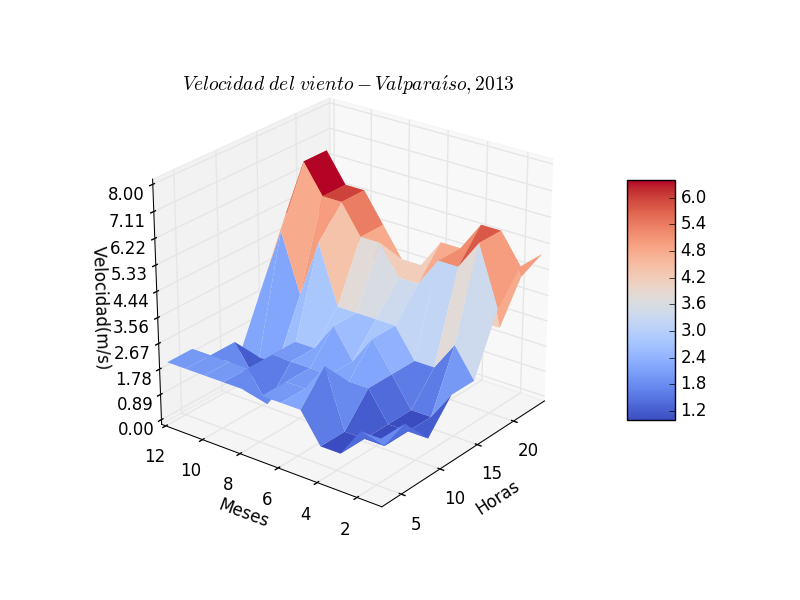
\includegraphics[width=0.4\textwidth]{figures/3d_data_2013.png}
        }%
         \subfigure[Vientos Valparaíso 2014.]{
            \label{fig:data_valpo_14}
            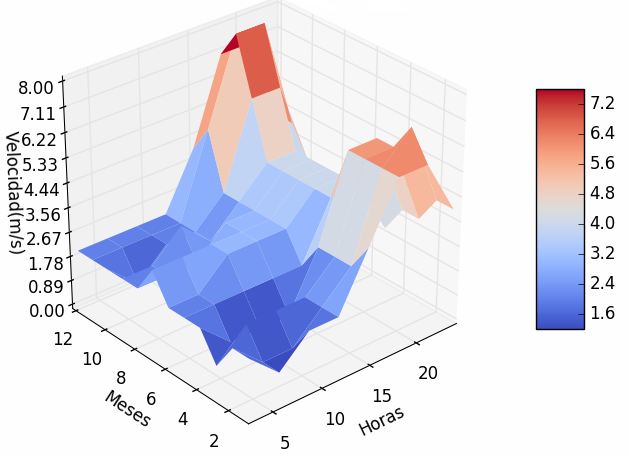
\includegraphics[width=0.4\textwidth]{figures/3d_data_2014.png}
        }\\
         \subfigure[Vientos Valparaíso 2015.]{
            \label{fig:data_valpo_15}
            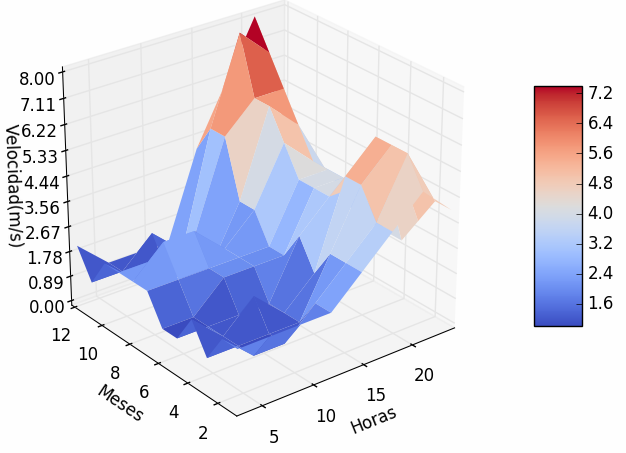
\includegraphics[width=0.4\textwidth]{figures/3d_data_2015.png}
        }%
    \caption{Superficie de datos viento de Valparaíso. Fuente: Elaboración Propia.}
    \label{fig:subfigures}
\end{figure}

\subsubsection{Experimento 1, datos anuales y promedios diarios}
Las figuras \ref{fig:pso_valpo_13}, \ref{fig:pso_valpo_14} y \ref{fig:pso_valpo_15} muestran el ajuste de la distribución de Weibull a los histogramas de datos del viento (promedios diarios), con los parámetros $k$ y $c$  que se muestran en las primeras tres filas de la tabla \ref{table:stadistical_tests} determinados por el PSO. El ajuste tiene buena forma, lo cual es corroborado por los datos estadísticos obtenidos con los test previamente mencionados (RMSE, r, RB), expuestos en la tabla \ref{table:stadistical_tests}. Si se compara con la precisión conseguida en el trabajo de Carneiro et al. \cite{Carneiro15}, se aprecia que el ajuste conseguido es levemente más impreciso, sobre todo en lo relativo al test RB. Esto podría deberse a la naturaleza de los datos 
trabajados.\\
\begin{figure}[ht!]
    \centering
        \subfigure[PSO Valparaíso 2013.]{
            \label{fig:pso_valpo_13}
            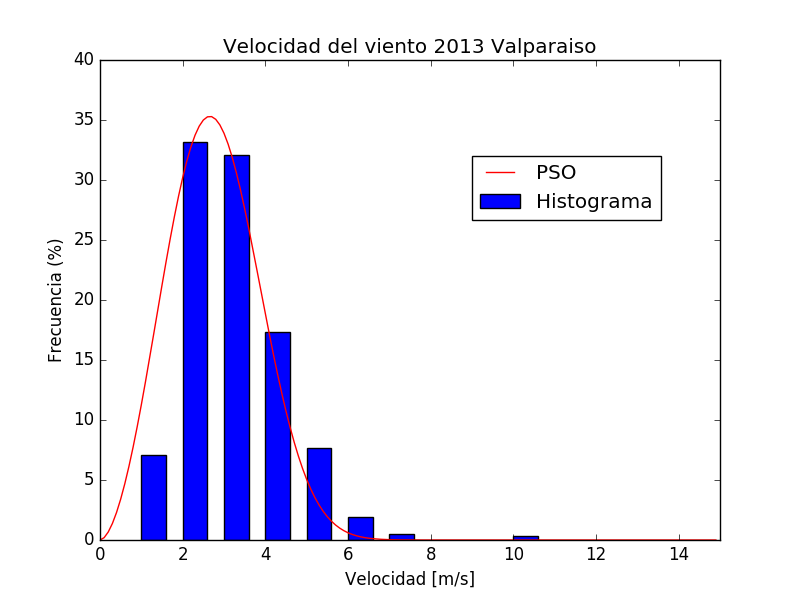
\includegraphics[width=0.4\textwidth]{figures/result_2013.png}
        }%
        \subfigure[PSO Valparaíso 2014.]{
            \label{fig:pso_valpo_14}
            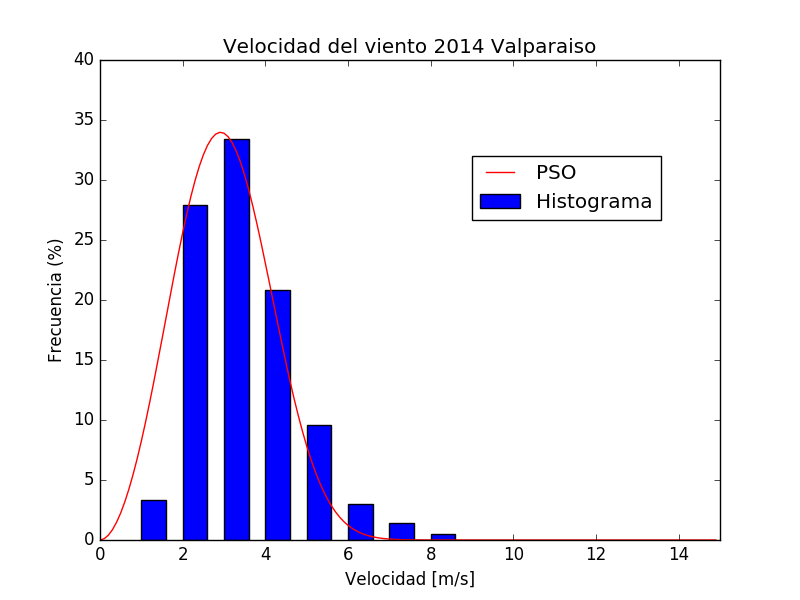
\includegraphics[width=0.4\textwidth]{figures/result_2014.png}
        }\\
        \subfigure[PSO Valparaíso 2015.]{
            \label{fig:pso_valpo_15}
            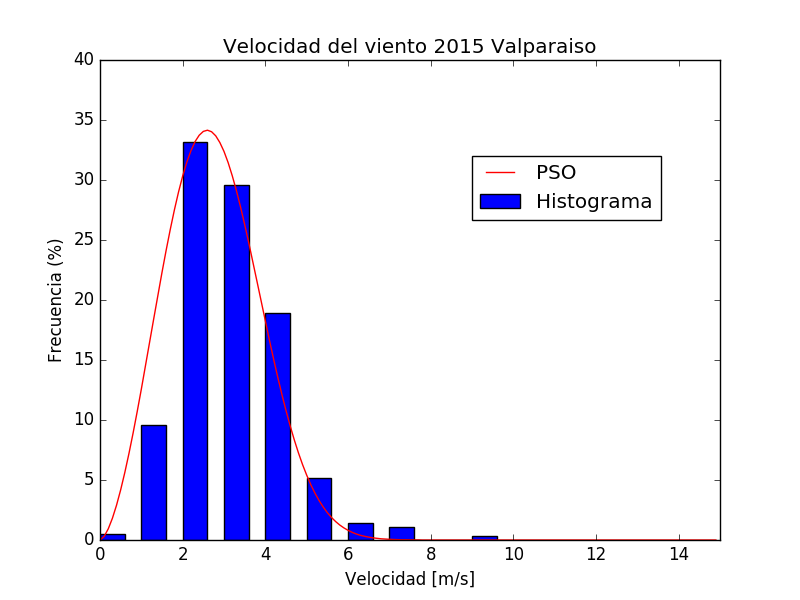
\includegraphics[width=0.4\textwidth]{figures/result_2015.png}
        }%
    \caption{Ajuste con PSO a datos del viento de Valparaíso. Fuente: Elaboración Propia.}
    \label{fig:subfigures}
\end{figure}

\subsubsection{Experimento 2, datos de tres años y promedios diarios}
En este experimento se realizó el ajuste considerando los promedios diarios y un intervalo de tres años consecutivos. El gráfico \ref{fig:pso_valpo_15_14_13_lq}, muestra el resultado del ajuste con PSO y la configuración estándar de los demás experimentos, es decir, 100 iteraciones y 50 partículas. En este gráfico se aprecia que el ajuste no es bueno, a pesar de las cifras en la tabla \ref{table:stadistical_tests}, fila 4: PSO (Intento 1), dado que oscila bastante alrededor de las barras del histograma, por lo que se repite el experimento aumentando el número de partículas a 200 obteniendo el gráfico \ref{fig:pso_valpo_15_14_13}, con el cual se obtiene un ajuste más adecuado, además de mejorar los resultados de los test estadísticos (tabla \ref{table:stadistical_tests}, fila 5: PSO (Intento 2)).\\
\begin{figure}[ht!]
    \centering
        \subfigure[Buen ajuste PSO Valparaíso 2013.]{
            \label{fig:pso_valpo_15_14_13}
            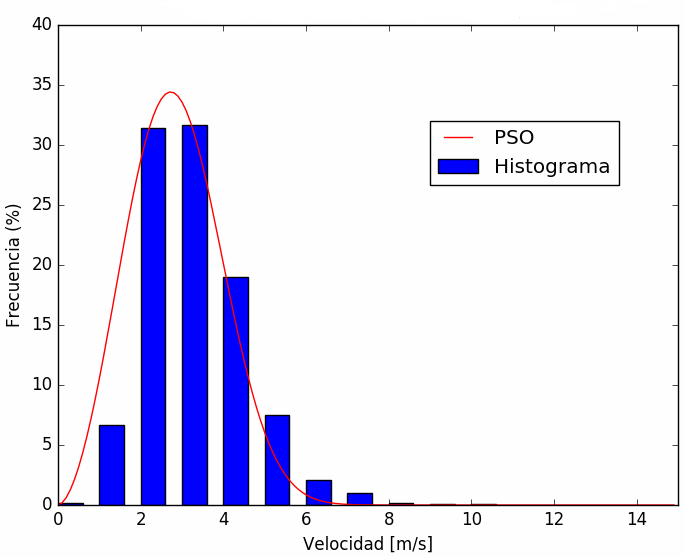
\includegraphics[width=0.4\textwidth]{figures/result_13-14-15.png}
        }%
        \subfigure[Mal ajuste PSO Valparaíso 2013.]{
            \label{fig:pso_valpo_15_14_13_lq}
            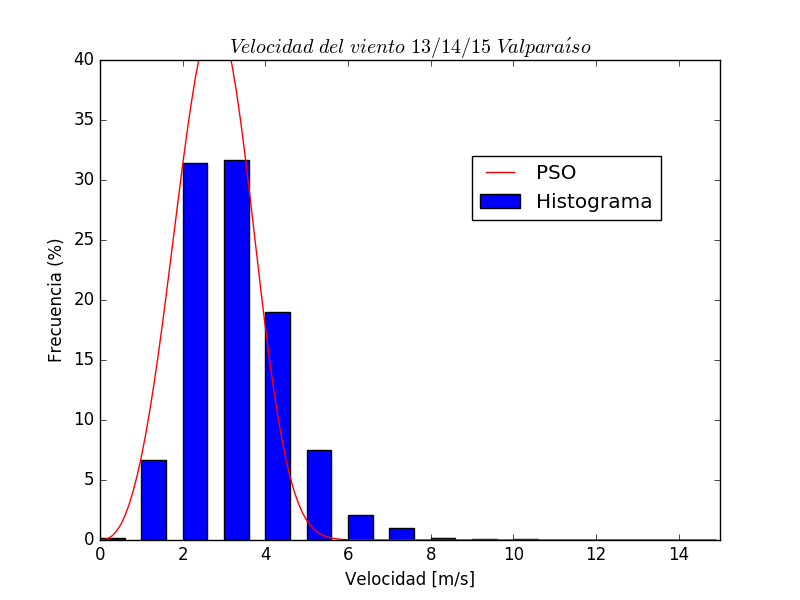
\includegraphics[width=0.4\textwidth]{figures/result_13-14-15_low_quality.png}
        }%
    \caption{Ajuste con PSO a datos Valparaíso 2015, 2014 y 2013, baja y buena calidad. Fuente: Elaboración Propia.}
    \label{fig:subfigures}
\end{figure}

\subsubsection{Experimento 3, ajuste a datos anuales con resultados del experimento 2}
Los gráficos \ref{fig:pso_valpo_13_all_data}, \ref{fig:pso_valpo_14_all_data} y \ref{fig:pso_valpo_15_all_data} son ajustes de Weibull con los parámetros obtenidos en el experimento anterior. Es decir, la idea es evaluar el modelo general de los tres años versus el histograma de datos de cada año en particular.
El ajuste desde los resultados estadísticos (tabla \ref{table:stadistical_tests}), es levemente menos preciso que el modelo ajustado a cada año en particular, pero sigue siendo aceptable como posible opción a considerar.
\begin{figure}[ht!]
    \centering
    \subfigure[Velocidad viento Valparaíso 2013.]{
        \label{fig:pso_valpo_13_all_data}
        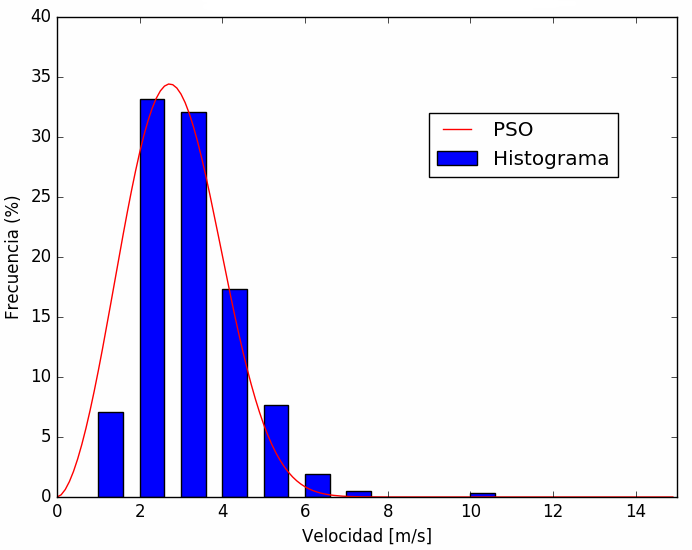
\includegraphics[width=0.4\textwidth]{figures/result_2013_fit_all_data.png}
    }%  
    \subfigure[Velocidad viento Valparaíso 2014.]{
        \label{fig:pso_valpo_14_all_data}
        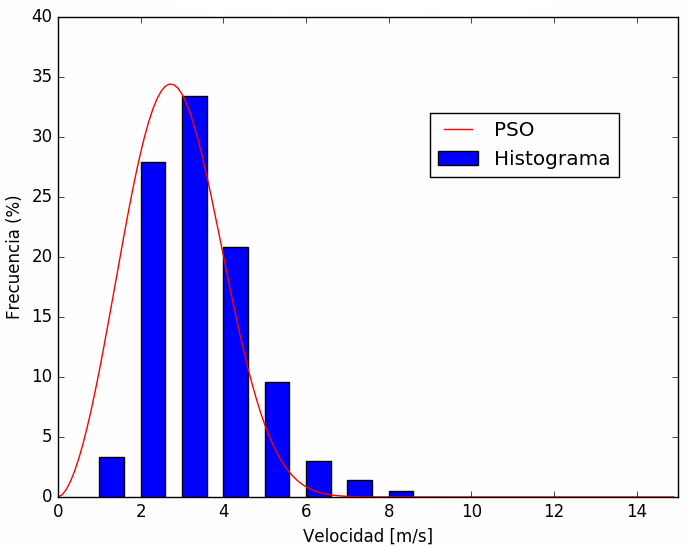
\includegraphics[width=0.4\textwidth]{figures/result_2014_fit_all_data.png}
    }\\   
    \subfigure[Velocidad viento Valparaíso 2015.]{
        \label{fig:pso_valpo_15_all_data}
        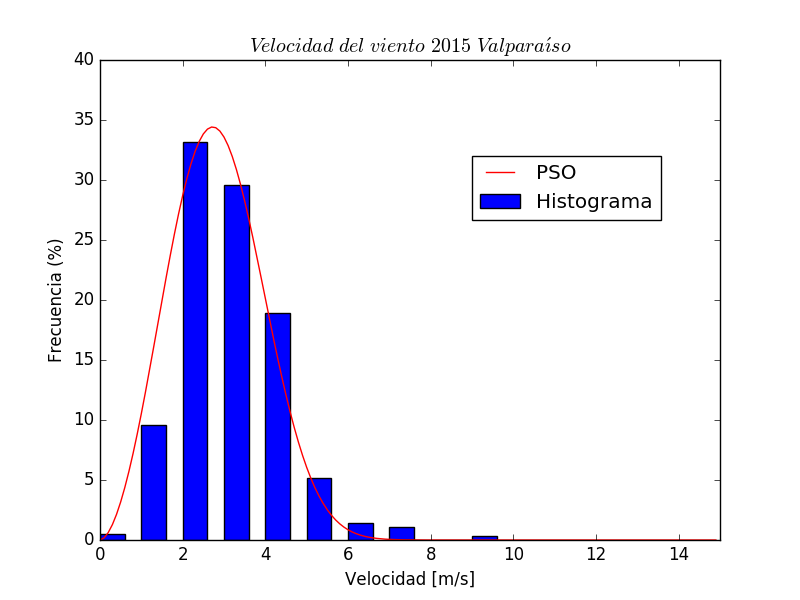
\includegraphics[width=0.4\textwidth]{figures/result_2015_fit_all_data.png}
    }%     

    \caption{Ajuste con PSO a registros del viento en Valparaíso (Con todos los datos). Fuente: Elaboración Propia.}
    \label{fig:subfigures}
\end{figure}

\subsubsection{Experimento 4, ajuste a datos de tres meses y promedios diarios}
Es posible que se requiera un análisis más acotado, por ello los gráficos \ref{fig:pso_valpo_15_ene_mar}, \ref{fig:pso_valpo_15_abr_jun}, 
\ref{fig:pso_valpo_15_jul_sep}, \ref{fig:pso_valpo_15_oct_dic}, muestran un ajuste considerando un lapso de 3 meses para el año 2015, con el
que se demuestra que es posible definir cualquier intervalo (manteniendo como unidad de dato el promedio diario de velocidad del viento)
 y obtener un ajuste adecuado de los datos mediante la distribución de Weibull.

\begin{figure}[ht!]
    \centering
    \subfigure[Enero - Marzo.]{
        \label{fig:pso_valpo_15_ene_mar}
        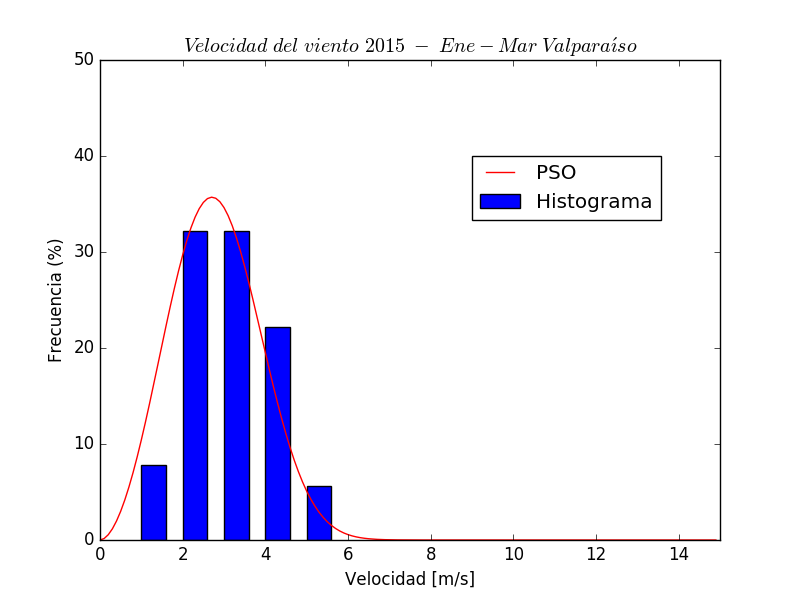
\includegraphics[width=0.4\textwidth]{figures/result_2015_Ene-Mar.png}
    }%  
    \subfigure[Abril - Junio.]{
        \label{fig:pso_valpo_15_abr_jun}
        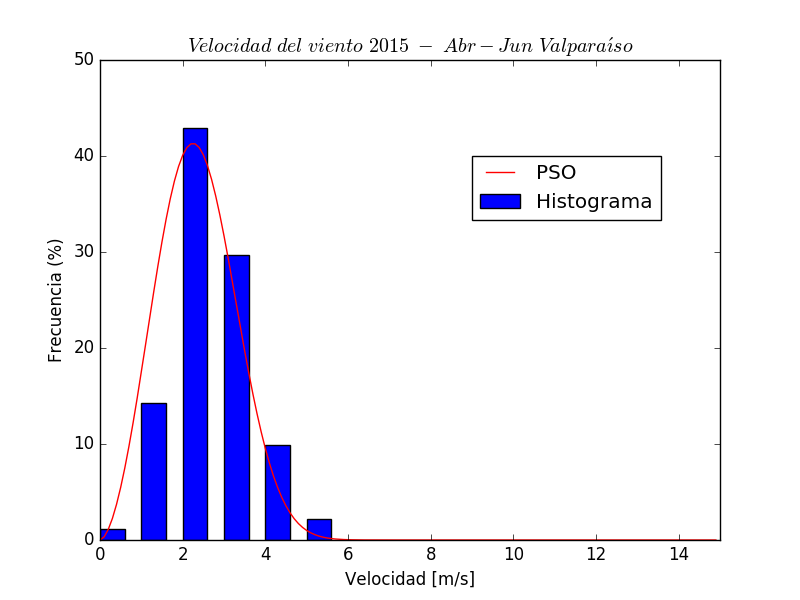
\includegraphics[width=0.4\textwidth]{figures/result_2015_Abr-Jun.png}
    }\\  
    \subfigure[Julio - Septiembre.]{
        \label{fig:pso_valpo_15_jul_sep}
        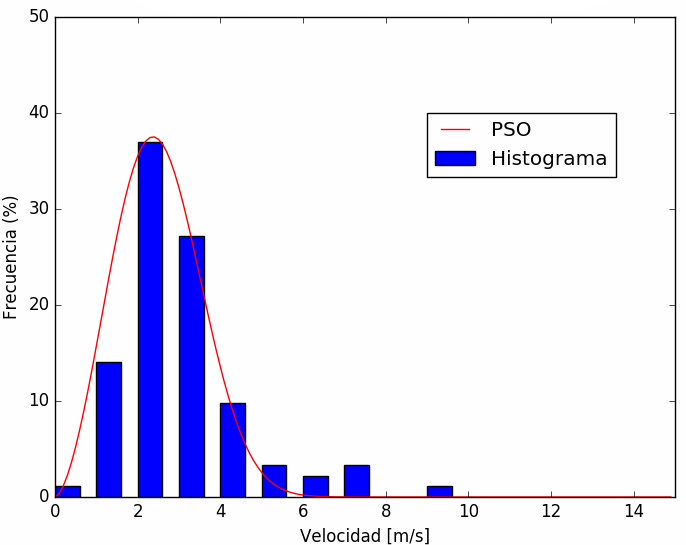
\includegraphics[width=0.4\textwidth]{figures/result_2015_Jul-Sep.png}
    }% 
    \subfigure[Octubre - Diciembre.]{
        \label{fig:pso_valpo_15_oct_dic}
        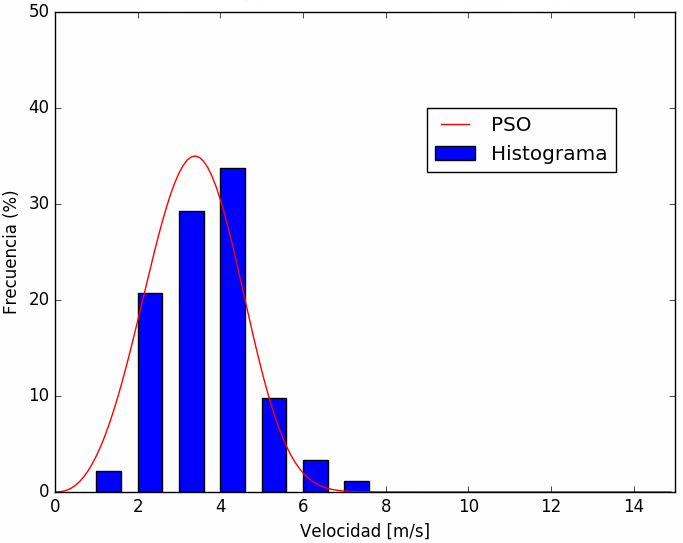
\includegraphics[width=0.4\textwidth]{figures/result_2015_Oct-Dic.png}
    }%  
    \caption{Ajuste con PSO a datos Valparaíso 2015, por rango de meses. Fuente: Elaboración Propia.}
    \label{fig:subfigures}
\end{figure}

\subsubsection{Experimento 4, ajuste a datos año 2015 y datos brutos}
La razón de por qué se utiliza el promedio diario de los datos del viento para ajustar Weibull y no las mediciones puras (las mediciones tomadas cada 3 horas diariamente) es expuesta en el gráfico \ref{fig:pso_valpo_15_all_data}. La distribución de Weibull no se ajusta a una distribución de datos con más de un máximo, por lo que de requerirse un modelo para este caso se debe buscar otra distribución o modificar Weibull.

\begin{figure}[ht!]
    \centering
    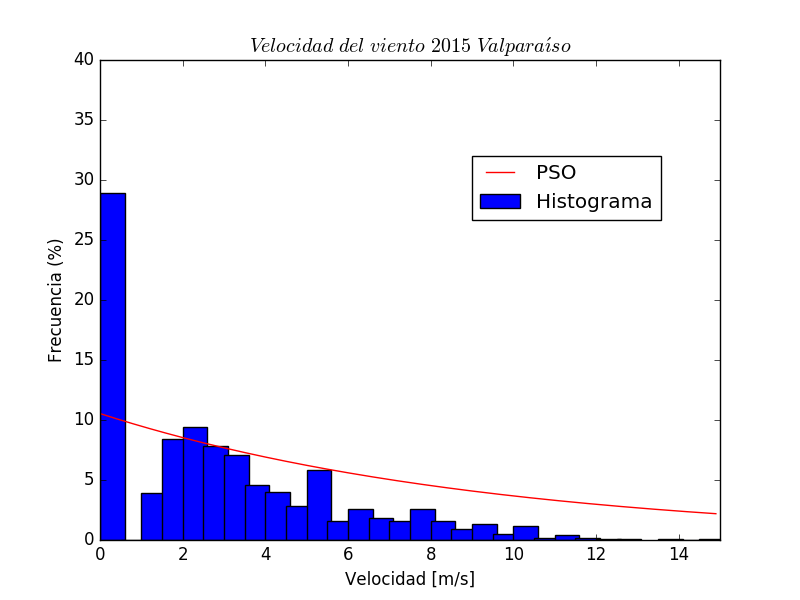
\includegraphics[width=0.4\textwidth]{figures/result_2015_all_data.png}
    \caption{Ajuste con PSO a datos (cifras puras) Valparaíso 2015, 2014, 2013}
    \vspace{-.25cm}
    \caption*{Fuente: Elaboración Propia.}
    \label{fig:pso_valpo_15_all_data}
\end{figure}

\subsubsection{Resumen de los experimentos}
\begin{table}[ht!]
    %\centering
    \caption{Tabla de tests estadísticos}
    \label{table:stadistical_tests}
    \resizebox{\textwidth}{!}{
    \begin{tabular}{|c|c|c|c|c|c|c|c|}
        \hline
        \textbf{\#} & \textbf{Método} & \textbf{Período} & \textbf{k} & \textbf{c} & \textbf{RMSE} & \textbf{r} & \textbf{RB}\\
        \hline
        1 & PSO & 2013 & 2.78 & 3.12 &0.0226585230791 & 0.984353070415 & 0.00197971468299\\
        2 & PSO & 2014 & 2.91 & 3.37 &0.0232779965263 & 0.982087745069 & 0.000754465101398\\
        3 & PSO & 2015 & 2.65 & 3.10 &0.0164721412159 & 0.992323803649 & 0.00302918178445\\
        \hline
        4 & PSO (Intento 1) & 2015-14-13 & 3.47 & 3.07 & 0.0360794587206 & 0.975240385258 & 0.000411212628513\\
        5 & PSO (Intento 2) & 2015-14-13 & 2.78 & 3.20 & 0.016175531561 & 0.994989105807 & 0.00190916669626\\
        \hline
        6 & PSO (Intento 2) & 2013 & 2.78 & 3.20 & 0.0240448436122 & 0.981963054492 & 0.00192186034284\\
        7 & PSO (Intento 2) & 2014 & 2.78 & 3.20 & 0.0301463089474 & 0.970662237238 & 8.89024791609e-05\\
        8 & PSO (Intento 2) & 2015 & 2.78 & 3.20 & 0.0202342934641 & 0.98662798667 & 0.00192175053173\\
        \hline
        9 & PSO & Ene-Mar & 2.85 & 3.15 & 0.0230380400157 & 0.982158006469 & 0.00641888742608\\
        10 & PSO & Abr-Jun & 2.76 & 2.65 & 0.0204300909755 & 0.993857185938 & 0.00303620481316\\
        11 & PSO & Jul-Sep & 2.66 & 2.83 & 0.0251002816356 & 0.985858767021 & 0.00443453471038\\
        12 & PSO & Oct-Dic & 3.40 & 3.75 & 0.0260278634297 & 0.978479679326 & 0.000716653529598\\
        \hline 
        13 & PSO (datos brutos) & 2015 & 1.00 & 9.49 & 0.0451794472583 & 0.751732944794 & 0.676094670465\\ 
        \hline
    \end{tabular}
    }   
\end{table}
\pagebreak
\subsection{Análisis de los resultados - dirección del viento}
\begin{figure}[ht!]
     \centering
        \subfigure[Evolucion de la solucion.]{
            \label{fig:EV_SOL}
            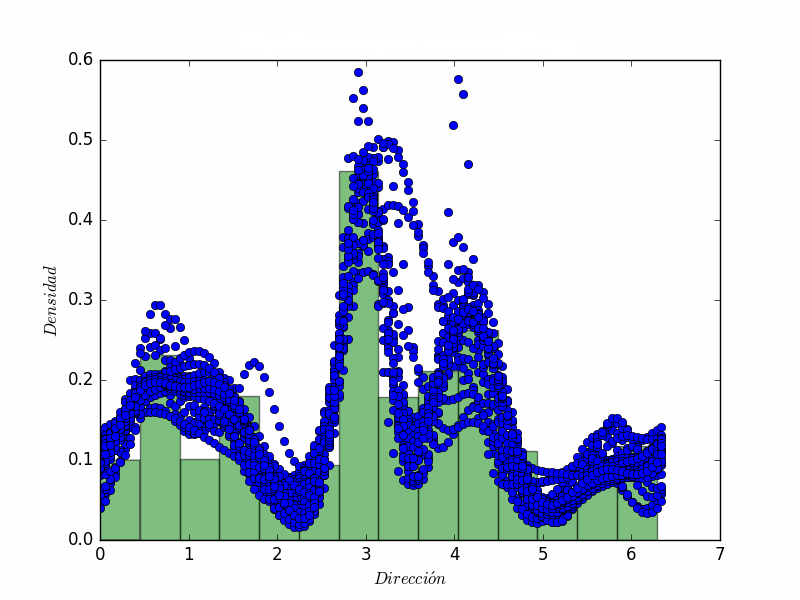
\includegraphics[width=0.4\textwidth]{figures/ev_solution.png}
        }%
        \subfigure[Comparacion solución inicial y final, 2015.]{
           \label{fig:COMP_INI_END}
           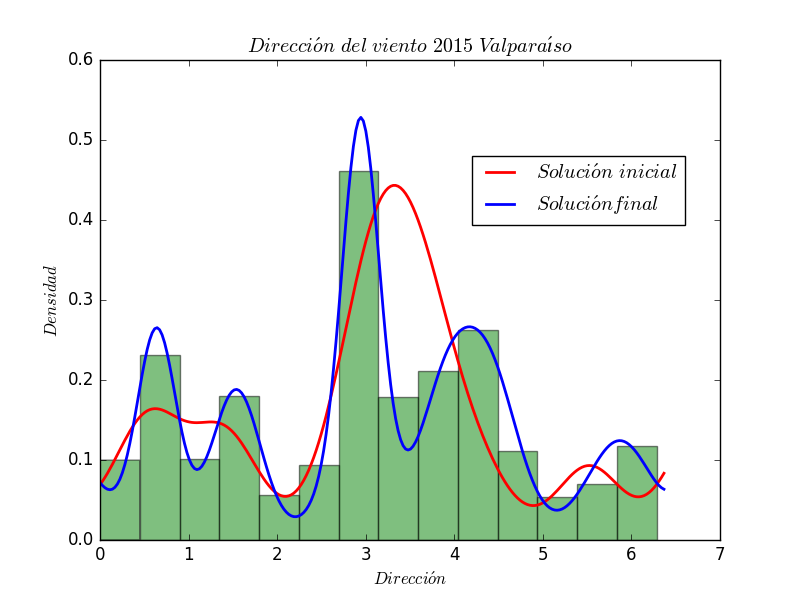
\includegraphics[width=0.4\textwidth]{figures/sol_ini_sol_fin.png}
        }\\ %  ------- End of the first row ----------------------%
        \subfigure[Ejemplo de mal ajuste, 2015.]{
            \label{fig:BAD_ADJUST}
            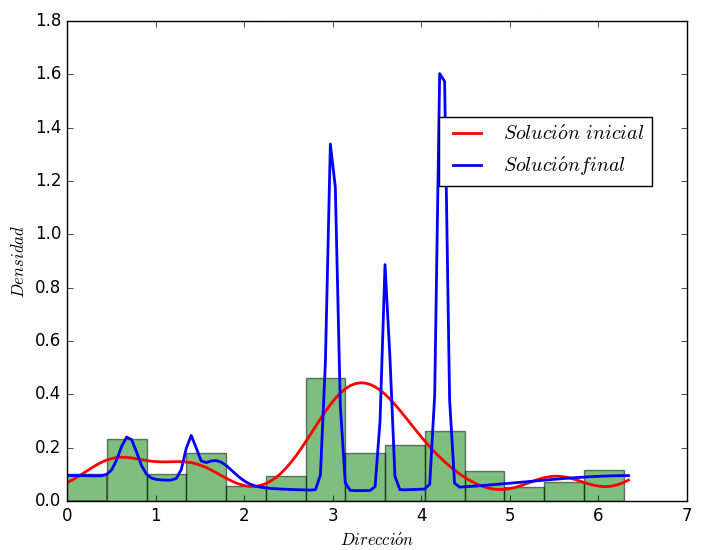
\includegraphics[width=0.4\textwidth]{figures/bad_adjust.png}
        }
        \subfigure[Solucion inicial y final, 2014.]{
            \label{fig:SOL_14}
            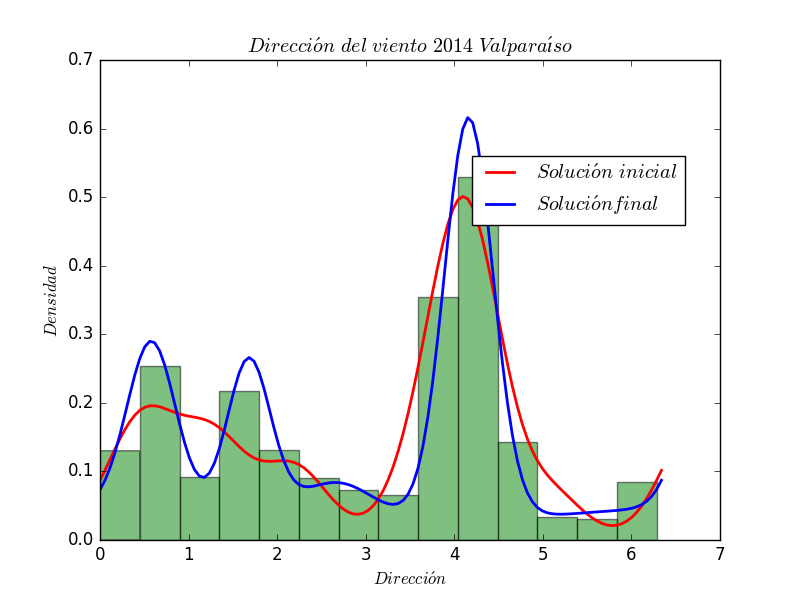
\includegraphics[width=0.4\textwidth]{figures/sol_ini_sol_fin_2014.png}
        }\\
         \subfigure[Solucion inicial y final, 2013.]{
            \label{fig:SOL_13}
            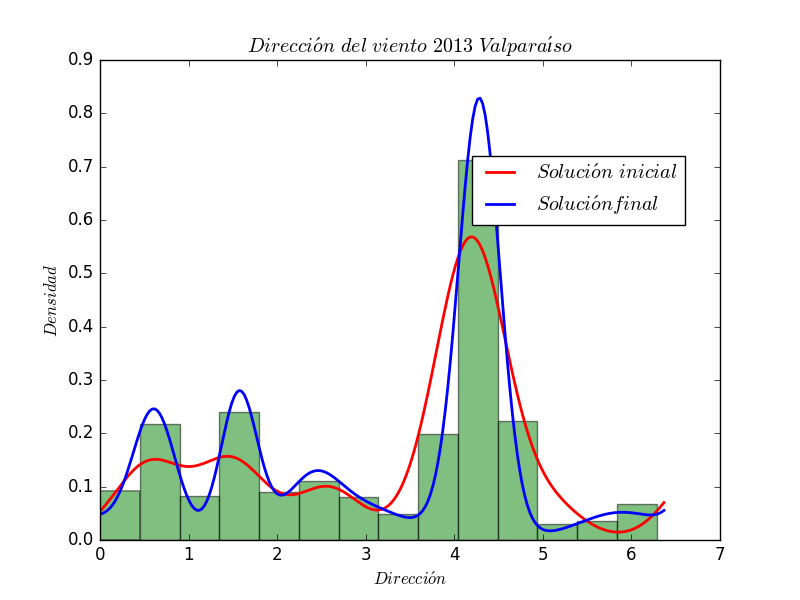
\includegraphics[width=0.4\textwidth]{figures/sol_ini_sol_fin_2013.png}
        }
    \caption{Graficos de ajustes anuales}
    \label{fig:subfigures}
\end{figure}
\begin{figure}[ht!]
    \begin{center}
         %%MONTHS  
        \subfigure[Solución inicial y final, Enero.]{
            \label{fig:PLOT_SOL_ENERO}
            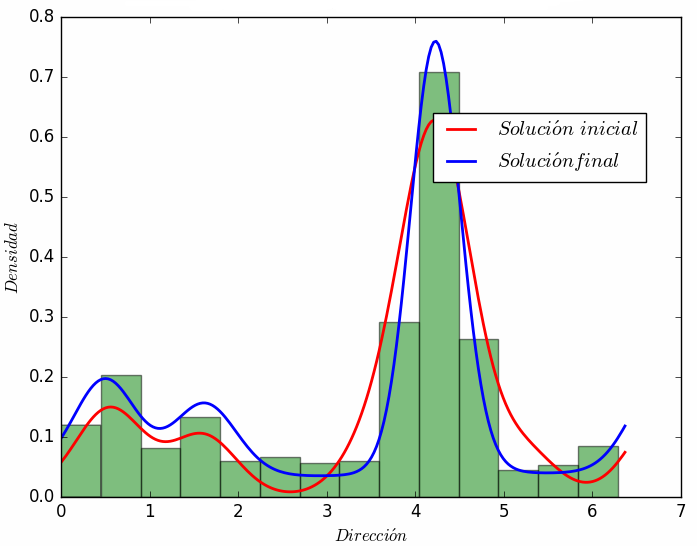
\includegraphics[width=0.4\textwidth]{figures/sol_ini_sol_fin_ENERO.png}
        }
         \subfigure[Solución inicial y final, Febrero.]{
            \label{fig:PLOT_SOL_FEBRERO}
            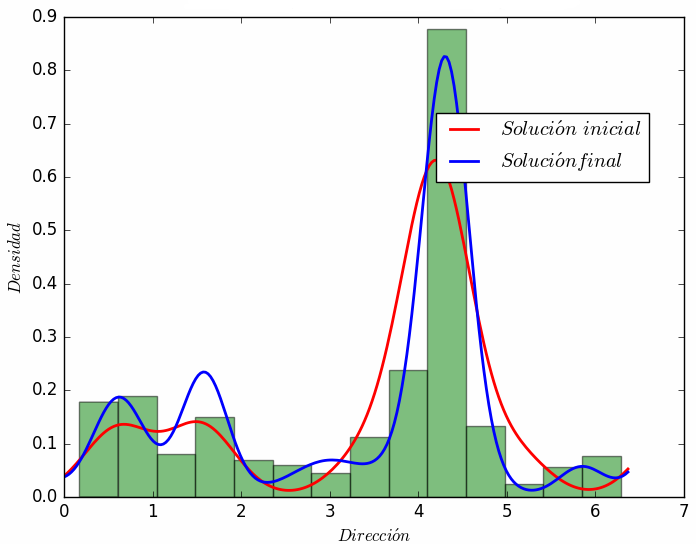
\includegraphics[width=0.4\textwidth]{figures/sol_ini_sol_fin_FEBRERO.png}
        }
          \subfigure[Solución inicial y final, Marzo.]{
            \label{fig:PLOT_SOL_MARZO}
            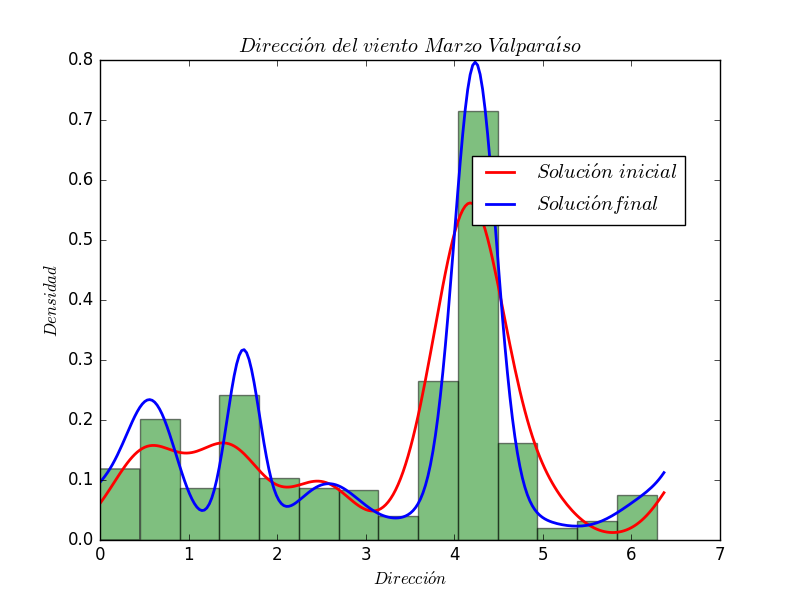
\includegraphics[width=0.4\textwidth]{figures/sol_ini_sol_fin_MARZO.png}
        }\\
         \subfigure[Solución inicial y final, Abril.]{
            \label{fig:PLOT_SOL_ABRIL}
            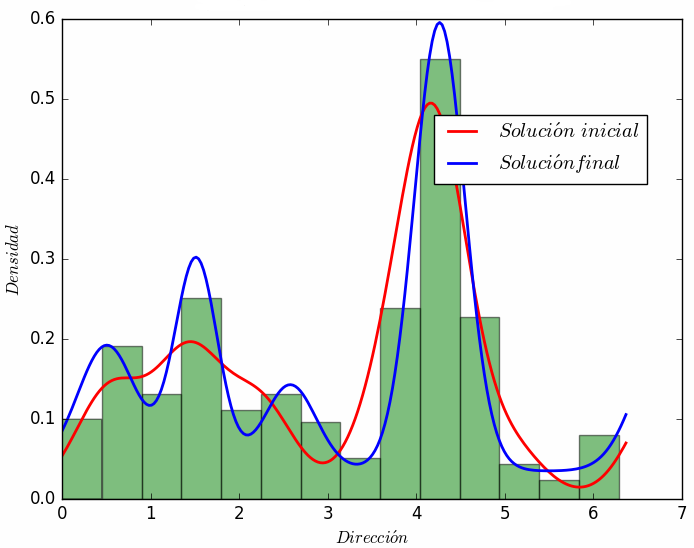
\includegraphics[width=0.4\textwidth]{figures/sol_ini_sol_fin_ABRIL.png}
        }
          \subfigure[Solución inicial y final, Mayo.]{
            \label{fig:PLOT_SOL_MAYO}
            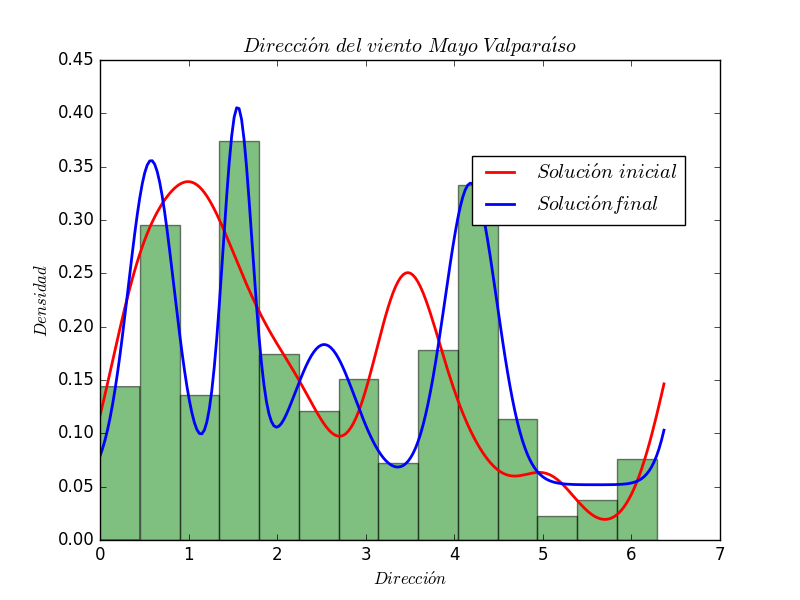
\includegraphics[width=0.4\textwidth]{figures/sol_ini_sol_fin_MAYO.png}
        }
         \subfigure[Solución inicial y final, Junio.]{
            \label{fig:PLOT_SOL_JUNIO}
            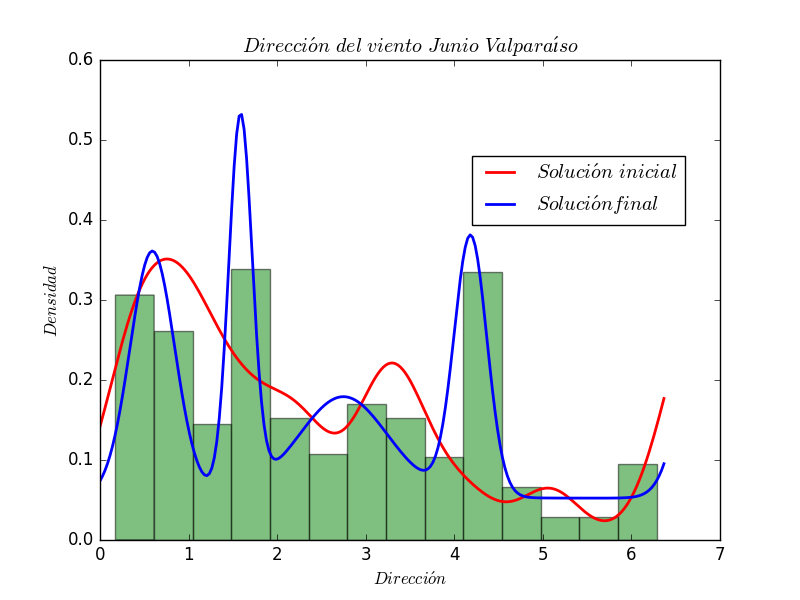
\includegraphics[width=0.4\textwidth]{figures/sol_ini_sol_fin_JUNIO.png}
        }
\end{center}
    \caption{Gráficos de ajuste de MVM por meses. Fuente: Elaboración propia.}
    \label{fig:PLOT_MONTHS}
\end{figure}

\begin{figure}[ht!]
    \begin{center}
        \subfigure[Solución inicial y final, Julio.]{
            \label{fig:PLOT_SOL_JULIO}
            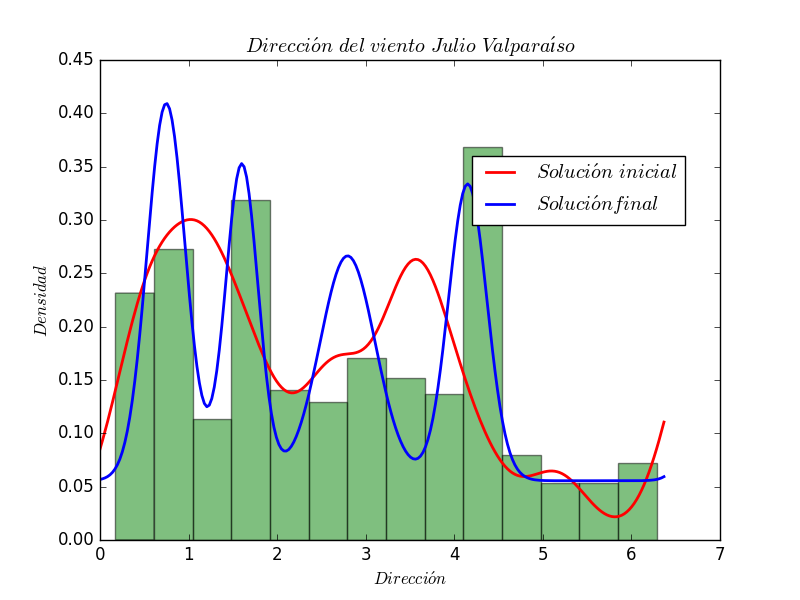
\includegraphics[width=0.4\textwidth]{figures/sol_ini_sol_fin_JULIO.png}
        }
         \subfigure[Solución inicial y final, Agosto.]{
            \label{fig:PLOT_SOL_AGOSTO}
            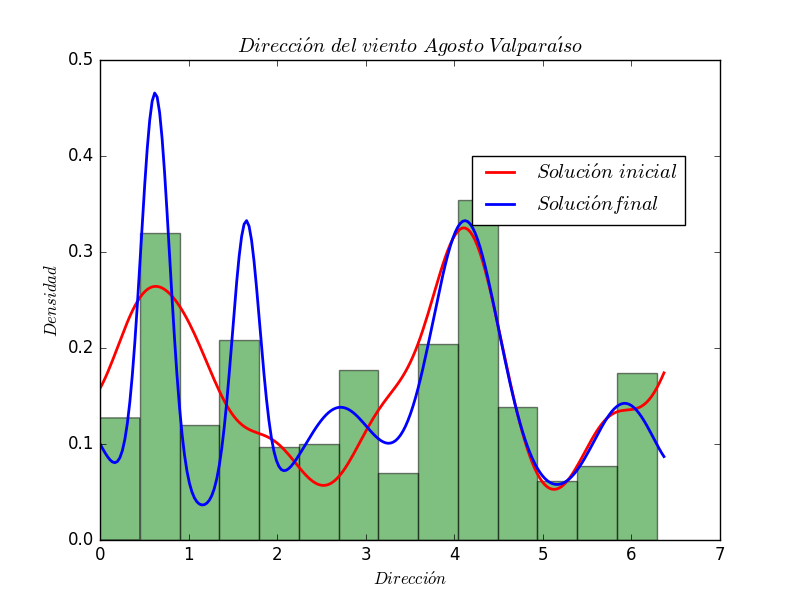
\includegraphics[width=0.4\textwidth]{figures/sol_ini_sol_fin_AGOSTO.png}
        }
          \subfigure[Solución inicial y final, Septiembre.]{
            \label{fig:PLOT_SOL_SEPTIEMBRE}
            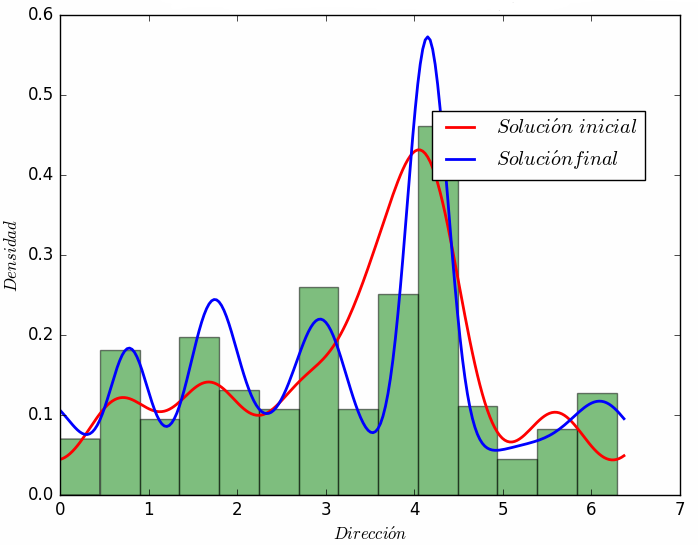
\includegraphics[width=0.4\textwidth]{figures/sol_ini_sol_fin_SEPTIEMBRE.png}
        }\\
         \subfigure[Solución inicial y final, Octubre.]{
            \label{fig:PLOT_SOL_OCTUBRE}
            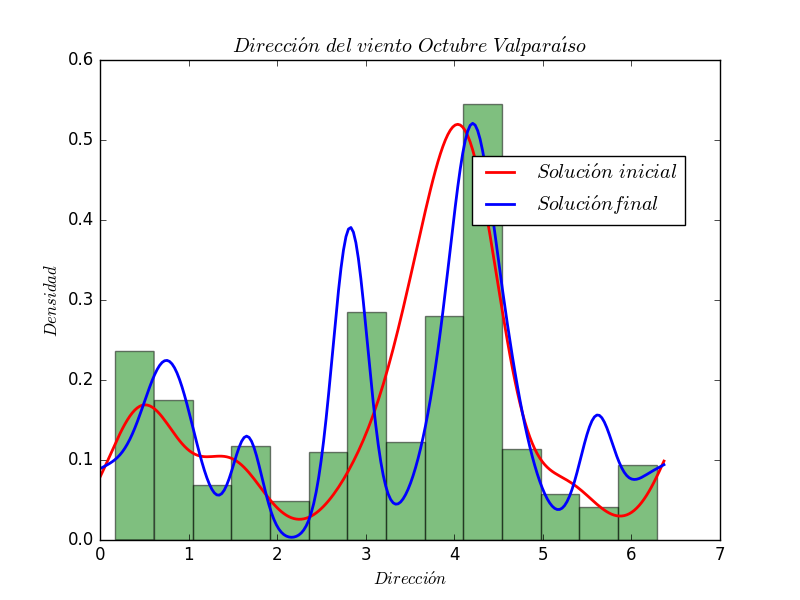
\includegraphics[width=0.4\textwidth]{figures/sol_ini_sol_fin_OCTUBRE.png}
        }
          \subfigure[Solución inicial y final, Noviembre.]{
            \label{fig:PLOT_SOL_NOVIEMBRE}
            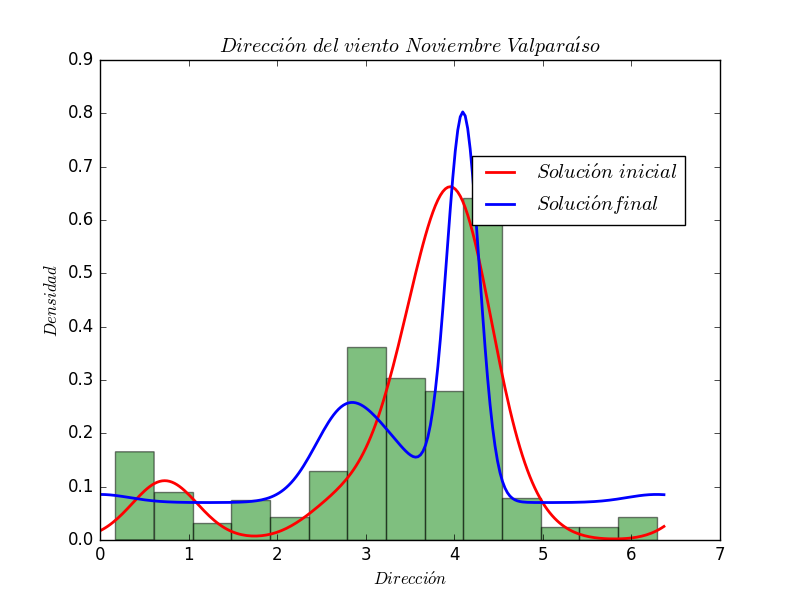
\includegraphics[width=0.4\textwidth]{figures/sol_ini_sol_fin_NOVIEMBRE.png}
        }
         \subfigure[Solución inicial y final, Diciembre.]{
            \label{fig:PLOT_SOL_DICIEMBRE}
            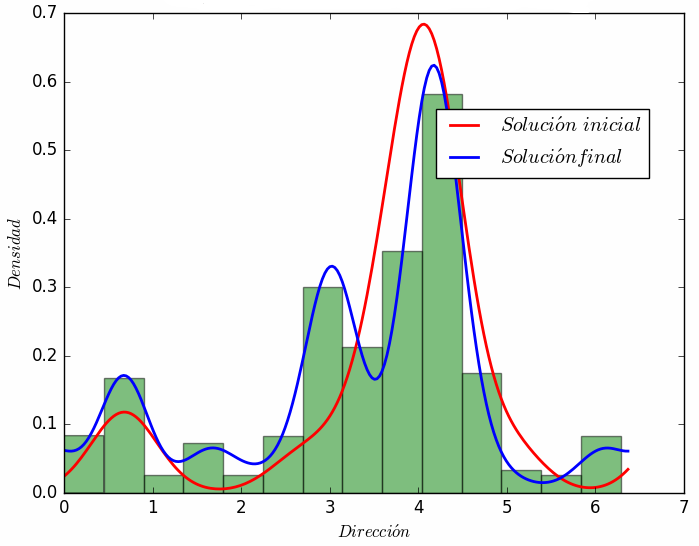
\includegraphics[width=0.4\textwidth]{figures/sol_ini_sol_fin_DICIEMBRE.png}
        }

    \end{center}
    \caption{Gráficos de ajuste de MVM por meses. Fuente: Elaboración propia.}
    \label{fig:PLOT_MONTHS}
\end{figure}

\pagebreak
\subsection{Conclusiones}
Para obtener información para alguna investigación relacionada a la velocidad del viento en una zona es necesario obtener un modelo que permita explicar las mediciones que se obtienen. Para ello, la distribución de Weibull es una de las funciones más utilizadas para el ajuste de los datos.
Distintos casos de estudio alrededor del mundo demuestran la utilidad de la distribución, utilizando diversos métodos para encontrar los parámetros de ajuste.
En este punto, la meta-heurística \emph{Particle Swarm Optimization} ha demostrado ser una alternativa eficiente para este problema, otorgando soluciones 
de alta calidad.\\
En este trabajo se presentó un caso de estudio para los datos del viento en Valparaíso, en donde los resultados muestran que la distribución de Weibull
se ajusta a la distribución de datos de promedios diarios de velocidad del viento. Esto quiere decir, que si estimamos la velocidad más probable, por ejemplo, 
esta se referirá al promedio más probable que se dé cierto día. Teniendo esto en cuenta, es posible obtener modelos para distintos intervalos de tiempo,
teniendo en cuenta que es posible modificar la calidad del modelos obtenido, mediante el ajuste de los parámetros de la distribución de Weibull.